\documentclass[11pt, aspectratio=169, compress]{beamer}
\usetheme[progressbar=frame title, numbering=fraction]{metropolis}      % Use metropolis theme 
\setbeamertemplate{section in toc}[sections numbered]
\setbeamertemplate{subsection in toc}[subsections numbered]
\useoutertheme[subsection=false]{miniframes}
\setbeamercolor{section in head/foot}{fg=white, bg=mDarkTeal}
\setbeamercolor{background canvas}{bg=white}
\setbeamerfont{section in head/foot}{series=\bfseries}

\usefonttheme[onlymath]{serif}
\usepackage{amsmath}
\usepackage{remreset}
\usepackage{ragged2e}
\usepackage{booktabs}
\usepackage{makecell}
\usepackage{float}
\usepackage{subfig}
\usepackage{tikz}
\usetikzlibrary{positioning,calc}
\usepackage[flushleft]{threeparttable}	% 3 part table 
\usepackage[justification=centering]{caption}
\captionsetup{skip=0pt}
\graphicspath{{./fig/}}

\makeatletter
\let\beamer@writeslidentry@miniframeson=\beamer@writeslidentry
\def\beamer@writeslidentry@miniframesoff{%
	\expandafter\beamer@ifempty\expandafter{\beamer@framestartpage}{}% does not happen normally
	{%else
		% removed \addtocontents commands
		\clearpage\beamer@notesactions%
	}
}
\newcommand*{\miniframeson}{\let\beamer@writeslidentry=\beamer@writeslidentry@miniframeson}
\newcommand*{\miniframesoff}{\let\beamer@writeslidentry=\beamer@writeslidentry@miniframesoff}
\beamer@compresstrue
\makeatother

%==============================================================
% Title Page
%==============================================================
%Information to be included in the title page:
\title{Economía social e instituciones (continuación)}
\author{Rony Rodriguez-Ramírez} 
\institute{Economía Social y Humana | Grupo B018 \\Universidad Centroamericana}
\titlegraphic{\hfill
\includegraphics[height=1.5cm]{uca}}
\date{\today}
%==============================================================
\begin{document}
	
\begin{frame}[plain]
	\maketitle  
\end{frame}

%\begin{frame}{Outline}
%\tableofcontents[hideallsubsections]
%\end{frame}
%------------------------------------------------
\section{Comentarios y anuncios}
%-----------------------------------------------
\subsection{Comentarios y anuncios}
%-----------------------------------------------
\begin{frame}{Comentario y anuncios}
\begin{itemize}
	\item Ensayo individual número 1: Resultados
	\begin{itemize}
		\item Media: 6.2 
		\item Mediana: 6 
		\item Max: 10 
		\item Min: 0
	\end{itemize}
	\item Errores generales del ensayo: Normas APA y enfoque de la tesis. 
	
\end{itemize}
\end{frame}
%------------------------------------------------
\begin{frame}{Comentario y anuncios}
\begin{columns}
	\begin{column}{0.5\textwidth}
		\begin{center}
		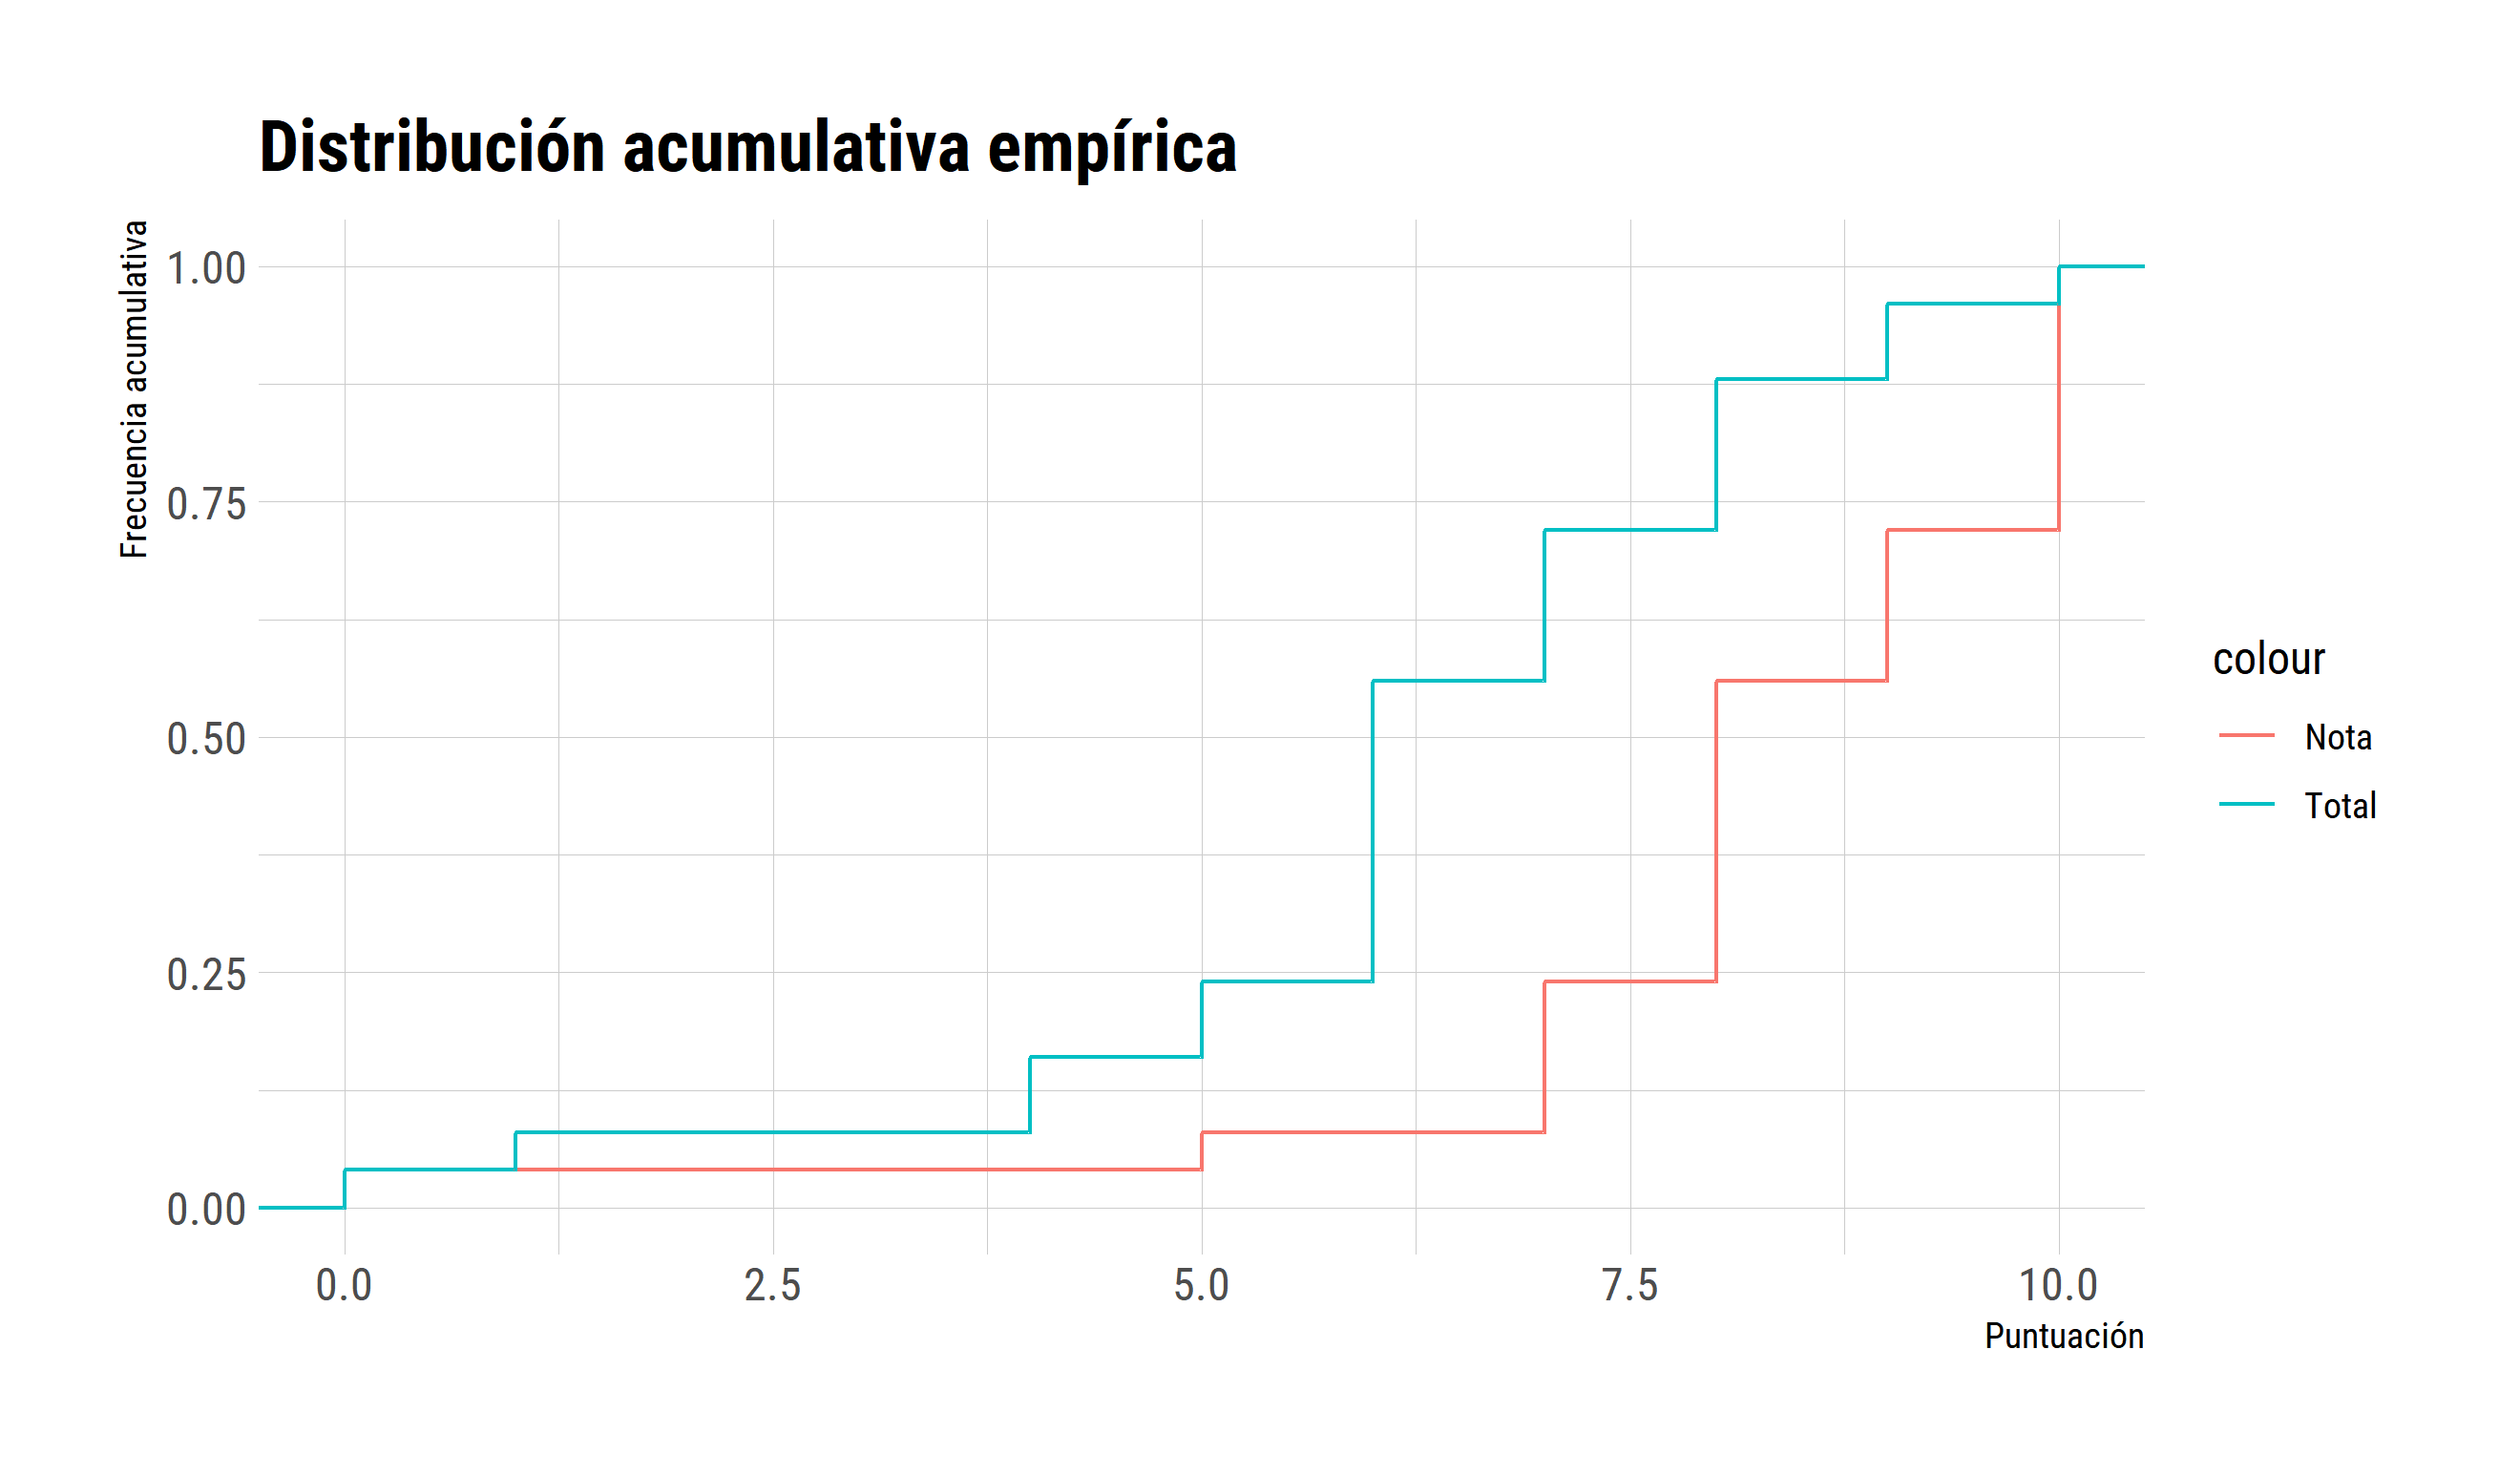
\includegraphics[width=1.1\textwidth]{fig1}
		\end{center}
	\end{column}
	\begin{column}{0.5\textwidth}  %%<--- here
		\begin{center}
			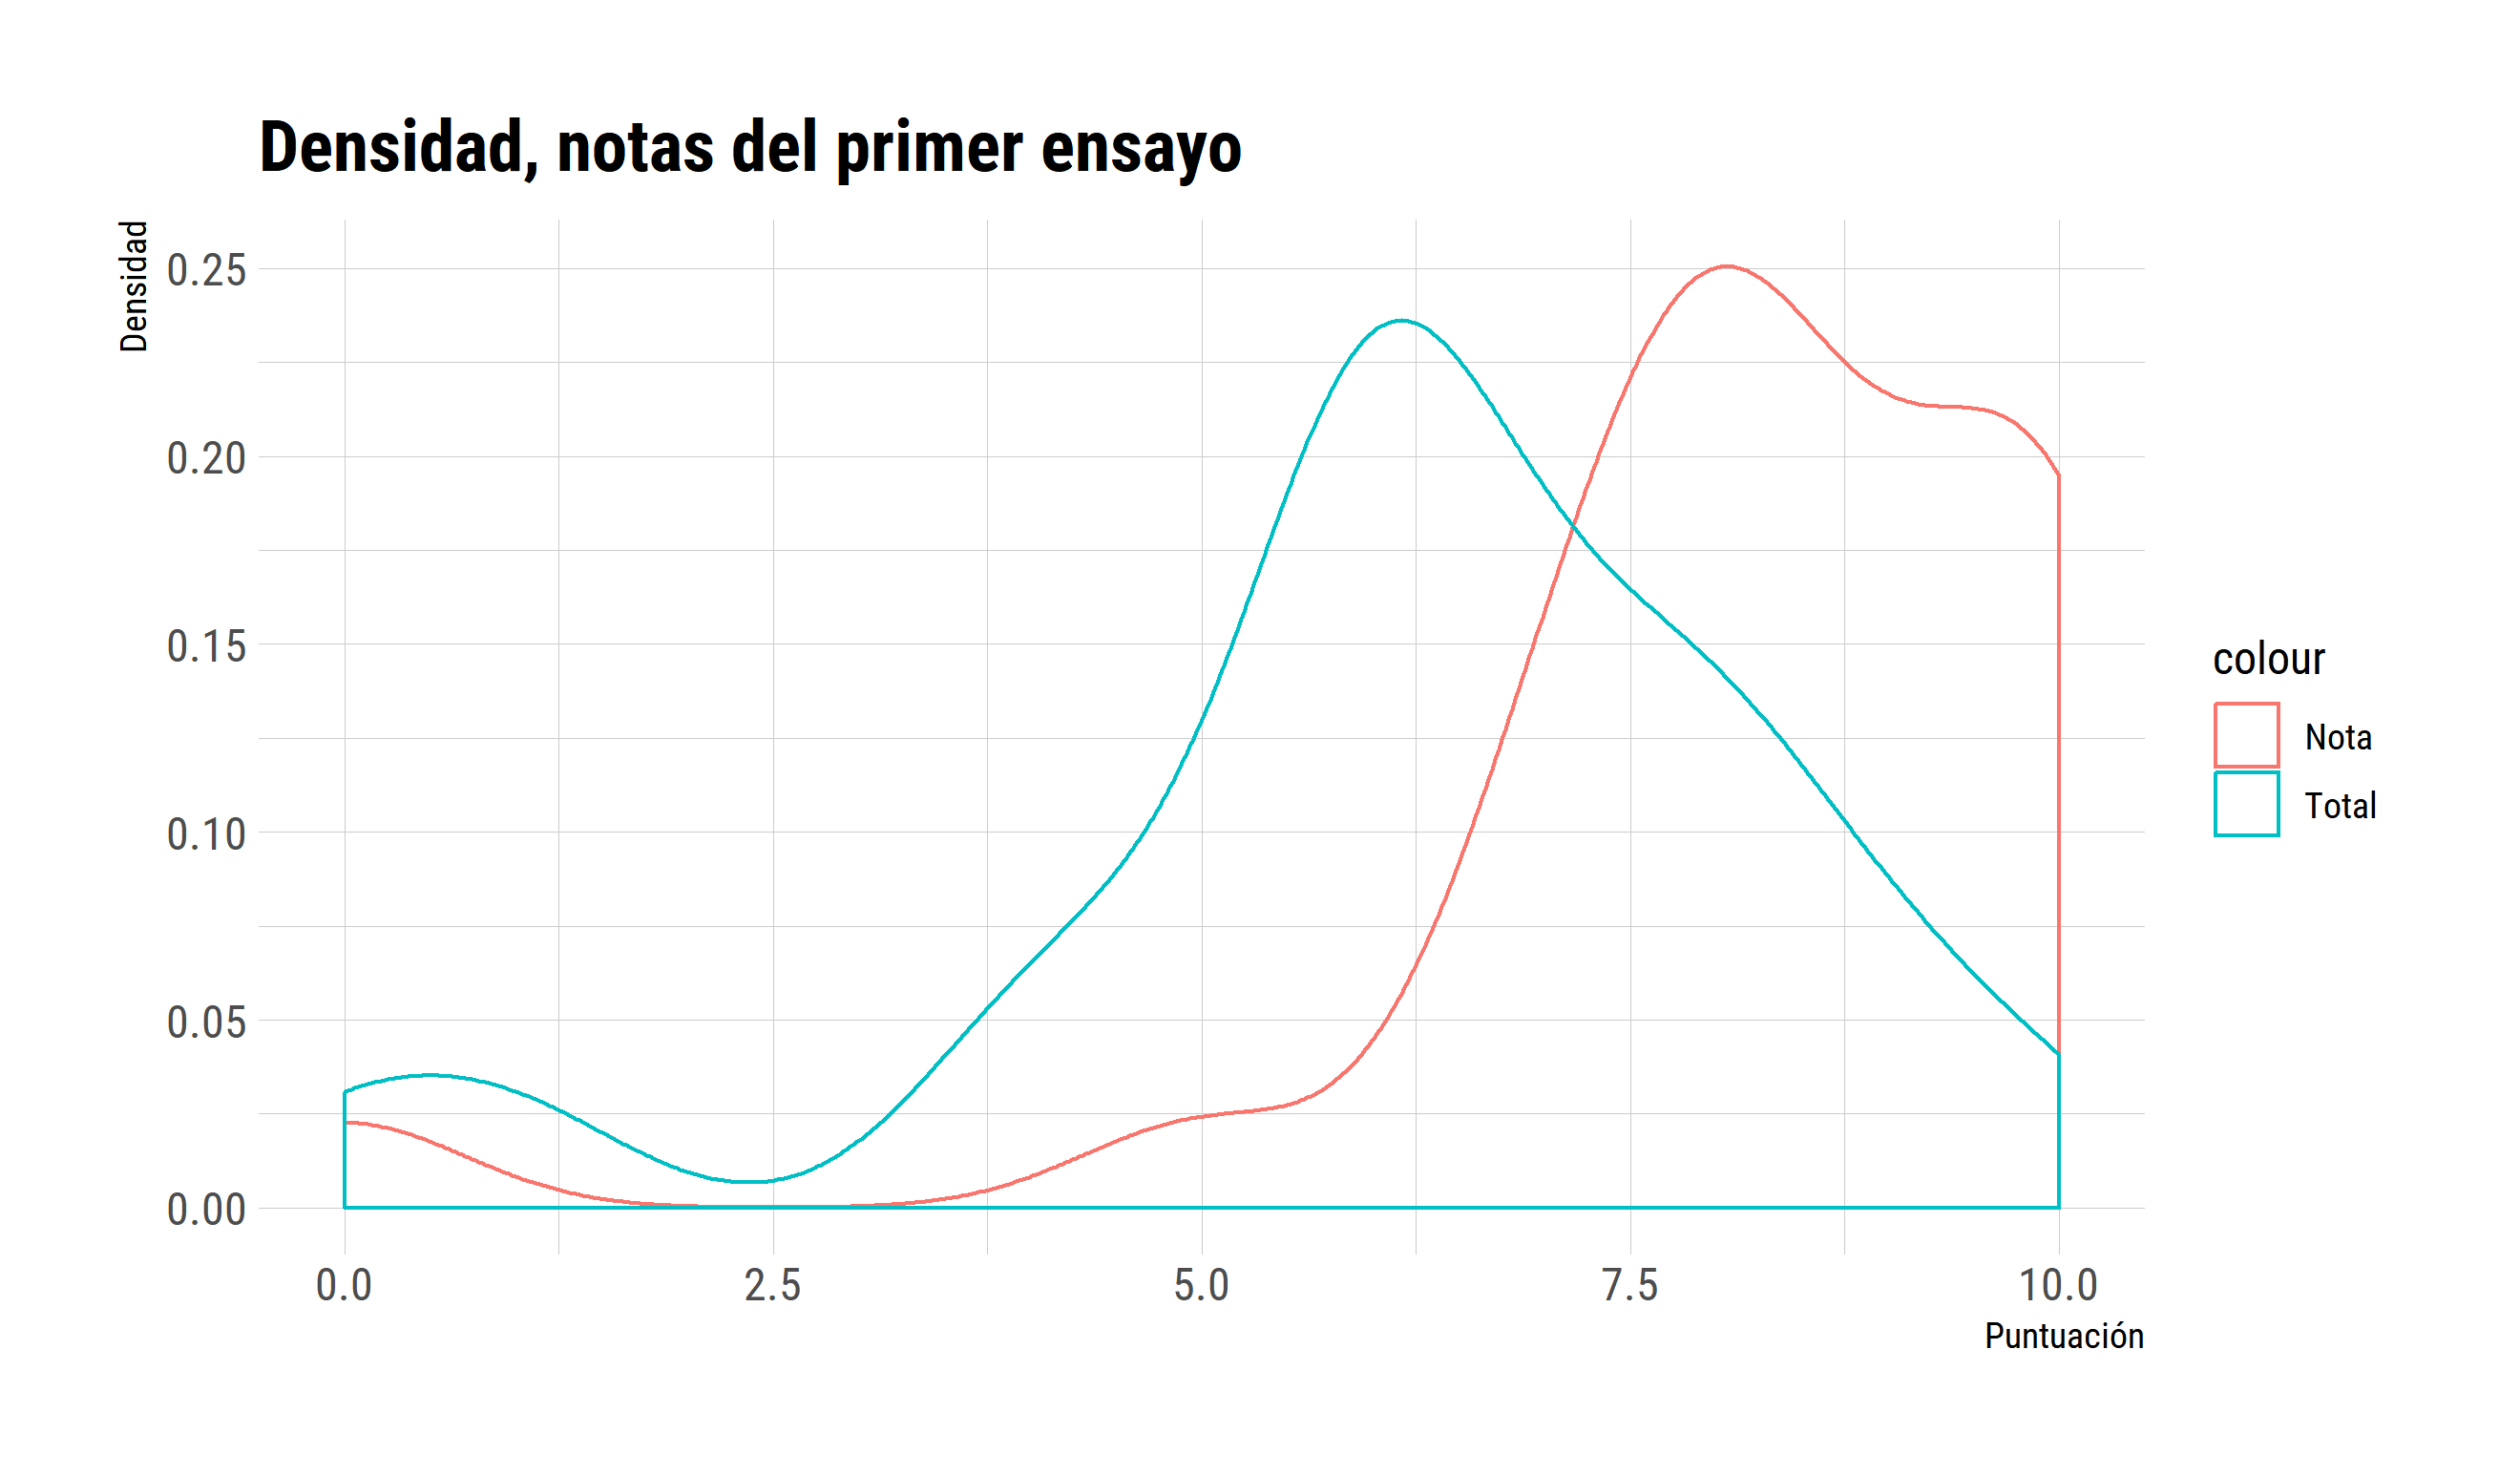
\includegraphics[width=1.1\textwidth]{fig2}
		\end{center}
	\end{column}
\end{columns}
\end{frame}
%------------------------------------------------
\section{Ostrom}
%-----------------------------------------------
\subsection{Ostrom}
%-----------------------------------------------
\begin{frame}{Reflexiones sobre los comunes}
	La tragedia de los comunes simboliza la degradaci'on del ambiente cuando muchos individuos utilizan por mucho tiempo un recurso escaso. 
	\begin{itemize}
	\item Esta conceptualización ha sido utilizada para describir casos de hambrunas, pastizales, sobrepoblación, los problemas de cooperación, etc. 
	\end{itemize}
\end{frame}
%------------------------------------------------
\begin{frame}{Reflexiones sobre el bienestar común}
	\begin{itemize}
		\item Es difícil lograr que los individuos persistan su bienestar común, en contraste con el individual (Olson, 1965). ¿Por qué? 
	\begin{itemize}
		\item El agumento es que si ``alguien que no puede ser exlcuído [...] de los beneficios [...] tiene poco incentivos para contribuir de manera voluntaria al suministro de ese bien" (Ostrom, 2000, pp. 31-32). 
	\end{itemize}
	\end{itemize}
\end{frame}
%------------------------------------------------
\begin{frame}{Relación con la lógica de la acción colectiva}
La tragedia de los comunes, el dilema del prisionera y la acción colectiva están altamente vinculados. 
\begin{itemize}
	\item No discutiremos a profundidad cada uno de ellos sino tomaremos en cuenta como se relacionan con la implementación de políticas y la economía social. 
\end{itemize}
\end{frame}
%------------------------------------------------
\begin{frame}{Prescripciones actuales de política}
	Existe el supuesto que es necesario un Leviatán; es decir, alguien externo con suficiente poder para evitar las tragedias de los comunes. Por ejemplo, el Estado, o consejos.
	\begin{itemize}
		\item Por lo general, esto sugiere que existe una entidad que decida las estrategias dentro de un esquema (juego).
		\item Un punto esencial acá es la información completa.  
		\item Sin información válidad y confliable, el Leviatán también cometerá errores. 
	\end{itemize} 
	También se encuentra la idea que la mejor forma de enfrentar estos problemas des a través de la privatización (Smith, 1981). 
\end{frame}
%------------------------------------------------
\begin{frame}{Reflexiones sobre los comunes}
	Sin embargo, es muy difícil decidir cuál via es la única vía posible para solucionar el problema de los comunes. 
	\begin{itemize}
		\item Para Ostrom (2000) existen muchan soluciones que enfrentarán muchos problemas distintos. 
		\item A su vez, sugiere opciones institucionales que puedan establecer contratos vinculantes para cooperación. 
	\end{itemize}
	En general, si se recomienda una única prescripción se estarían simplificando la diversidad de los problemas de los comunes. 
\end{frame}
%------------------------------------------------
\section{Nunn \& Wantchekon (2011)}
%-----------------------------------------------
\subsection{Nunn \& Wantchekon}
%-----------------------------------------------
\begin{frame}{Introducción}
Desde los siglos XVI al XIX, miles de esclavos fueron capturado y enviado a través del Océano Atlántico al ``Nuevo Mundo''": 
\begin{itemize}
	\item Nunn (2008) complied data on 80K slaves sold in the Atlantic
	trade, and 21K sold in the Indian trade between 1400 and 1900.
\end{itemize}
El comercio de esclavos tuvo un gran impacto en el tejido social de la sociedad africana, especialmente a fines del siglo XIX: 
\begin{itemize}
	\item  Inicialmente, esclavos capturados a través de incursiones organizadas por el estado y la guerra. 
	\item Mayor ambiente inseguridad ubicua $ \rightarrow $ los individuos se volvieran contra amigos y familiares (Nunn \& Wantchekon, 2011). 
\end{itemize}
\end{frame}
%-----------------------------------------------
\begin{frame}{Introducción}
En este entorno, puede haber evolucionado una cultura de desconfianza, que puede persistir hasta nuestros días.
\begin{itemize}
	\item El hecho de que los esclavos a menudo fueron llevados o engañados como esclavos por personas cercanas a ellos sugiere que el comercio de esclavos puede haber erosionado la confianza incluso en las relaciones sociales más íntimas.
\end{itemize}
\end{frame}
%-----------------------------------------------
\begin{frame}{Pregunta e hipótesis de investigación}
\textbf{Pregunta de la investigación: }
\begin{itemize}
	\item ¿El comercio de esclavos causó una cultura de desconfianza entre las etnias africanas?
\end{itemize}
\textbf{Hipótesis: }
\begin{itemize}
	\item Las personas que pertenecen a grupos étnicos que fueron más expuestos a los traficantes de esclavos exhiben niveles más bajos de confianza en sus familiares, vecinos, familias y gobiernos locales en la actualidad; esta cultura de desconfianza perdura hasta hoy, 
\end{itemize}
\end{frame}
%-----------------------------------------------
\begin{frame}{Estrategia de identificación}
\textbf{Datos: }
\begin{itemize}
	\item Afrobarometer 2005: 
	\item Nunn (2008): estimaciones sobre el número de esclavos. 
\end{itemize}
\end{frame}
%-----------------------------------------------
\begin{frame}{Estrategia de identificación}
OLS: 
\begin{equation}
	trust_{i,e,d,c} = \alpha_c + \beta slave~exports_e + \mathrm{\text{X'}}_{i,e,d,c,}\Gamma + \mathrm{\text{X'}}_{d,c,}\omega + \mathrm{\text{X'}}_{e}\Phi + \varepsilon_{i,e,d,c}
\end{equation}

\begin{itemize}\small
	\item $ i = $ individuo, $ e = $ grupo étnico, $ d = $ distrito, $ c = $ país. 
	\item $ slave~exports $ es una medida del número de esclaves de un grupo étnico. 
	\item Vector de controles por: edad, edad al cuadrado, género, localización, 5 efectos fijos de las condiciones de vida, 10 efectos fijos sobre educación, 18 efectos fijos de region, y 25 de ocupación. 
	\item Vector de controles por fractionalización de un distrito, y población de un distrito. 
	\item Vector de controles al nivel de etnicidad para capturar characterísticas históricas. 
\end{itemize}
\end{frame}
%-----------------------------------------------
\begin{frame}{Resultados}
\begin{figure}[htb]
	\centering
	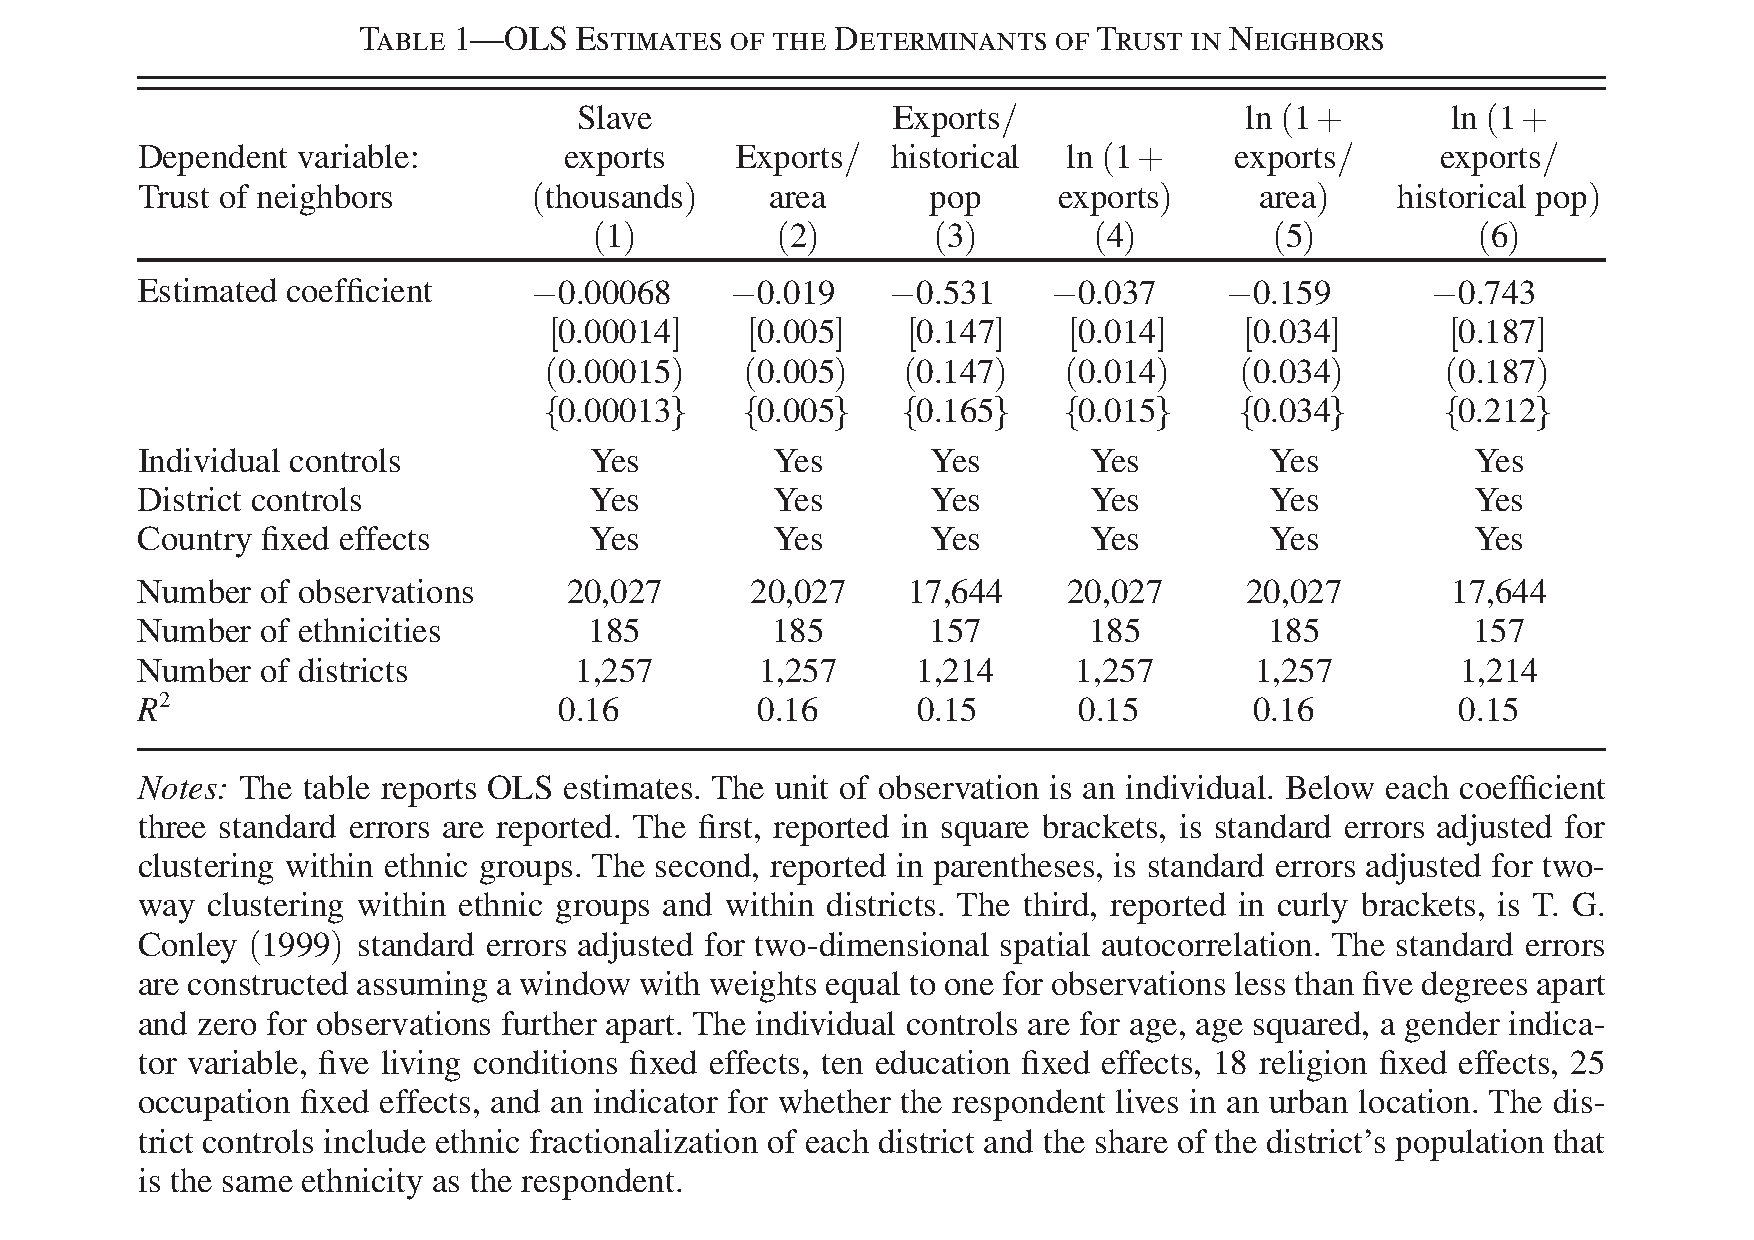
\includegraphics[width=.7\textwidth]{tab1}
\end{figure}
\end{frame}
%-----------------------------------------------
\begin{frame}{Resultados}
	\begin{figure}[htb]
		\centering
		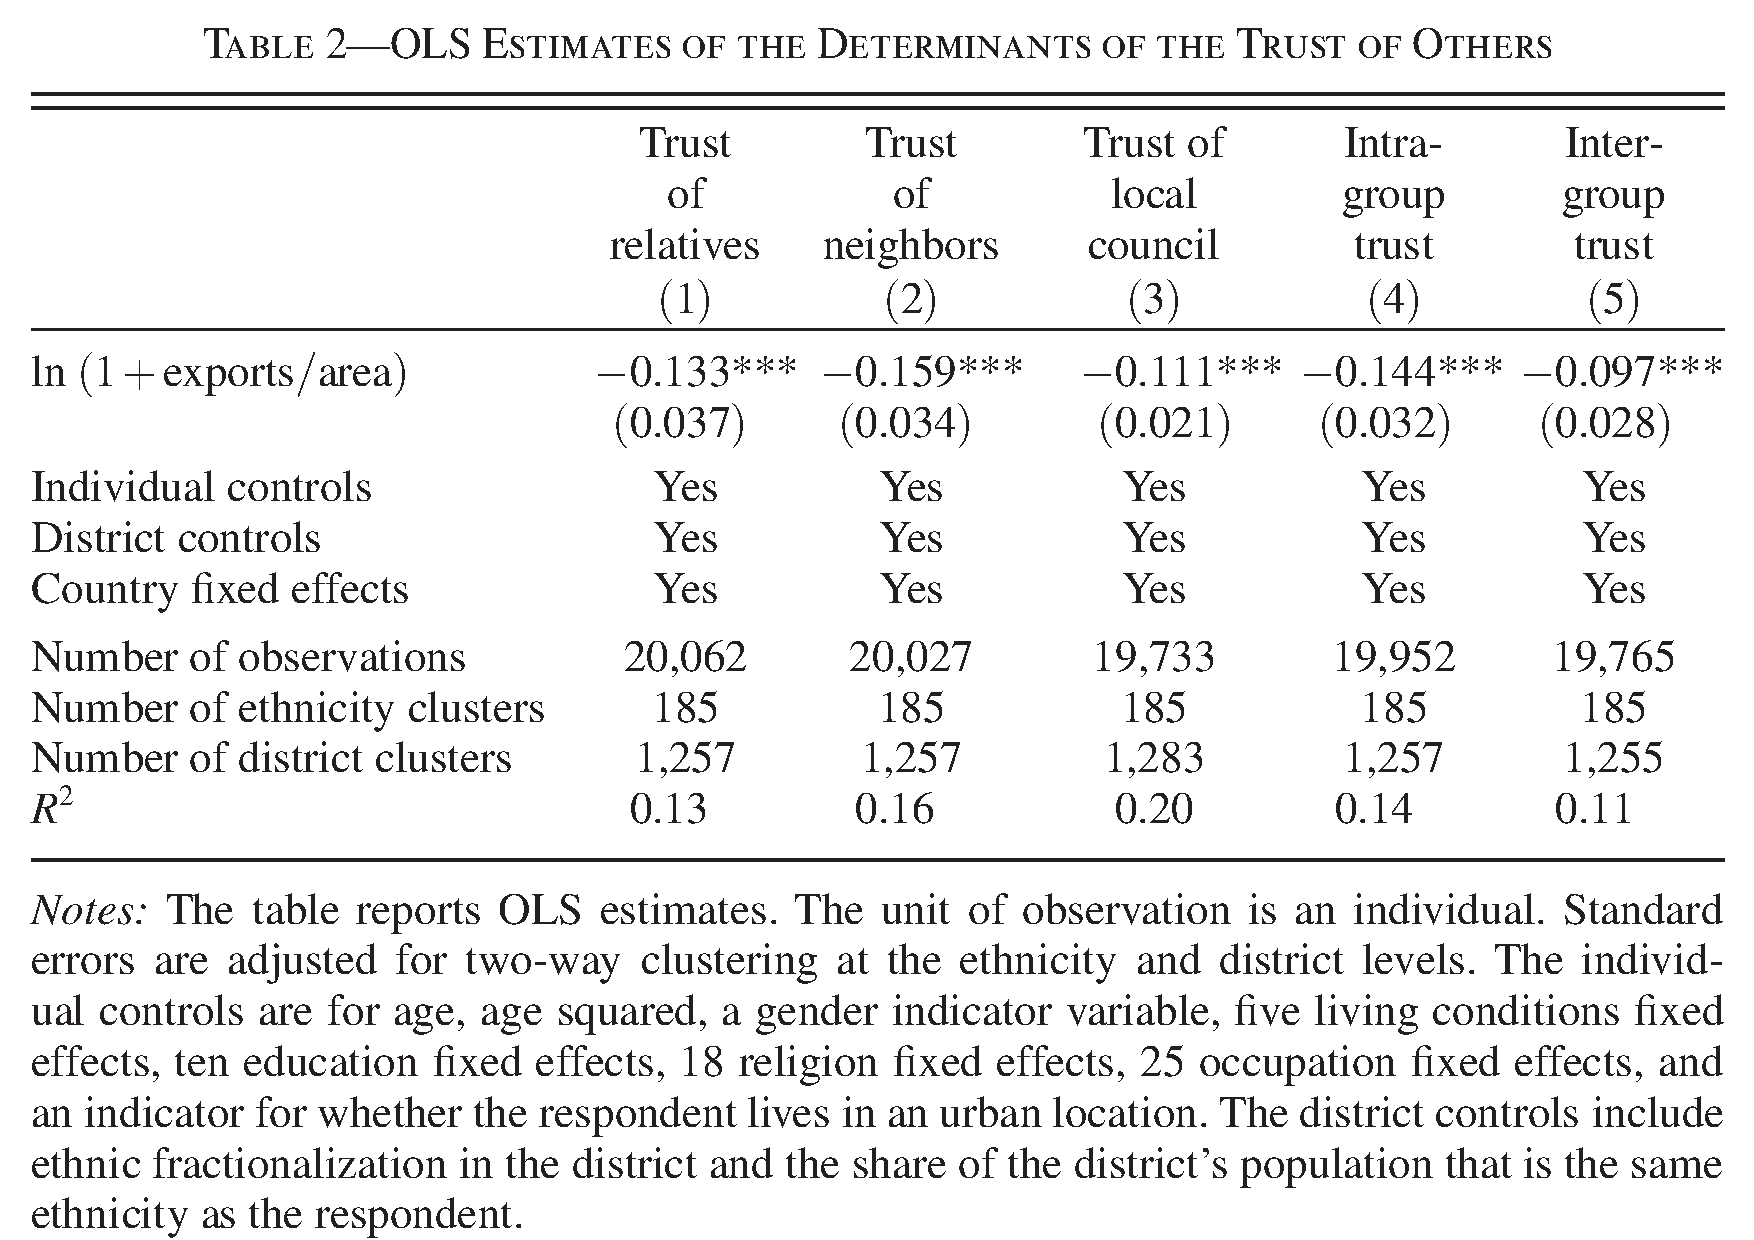
\includegraphics[width=.7\textwidth]{tab2}
	\end{figure}
\end{frame}
%-----------------------------------------------
\begin{frame}{Mecanismo causal}
Estas correlaciones podrían explicarse de otras maneras.
\begin{itemize}
	\item Los grupos que eran intrínsecamente menos confiados tenían más probabilidades de ser tomados durante el comercio de esclavos, y continúan siendo menos confiados en la actualidad.
	\item Otros eventos históricos: e.g., regla colonial, pueden estar correlacionadas con el comercio de esclavos y tienen un efecto directo en la confianza. 
\end{itemize}
\end{frame}
%-----------------------------------------------
\begin{frame}{Mecanismo causal}
	Por lo tanto, los autores: 
	\begin{itemize}
		\item Controlan por factores que determinan instituciones coloniales: malaria, ingreso pre-colonial (densidad poblacional etc.), influencia europea. 
		\item Los resultados en general no cambian y se mantiene la relación negativa. 
	\end{itemize}
\end{frame}
%-----------------------------------------------
\begin{frame}{Otra estrategia: Utilizar una variable instrumental}
Instrumento: 
\begin{itemize}
	\item Distancia a la costa: es plausiblemente no correlacionada con otros factores que afectan a la confianza de los descendientes de las etnicas de los esclavos. 
	\item No hay razón para creer que grupos menos confiados vivían cerca de la costa. 
\end{itemize}
\end{frame}
%-----------------------------------------------
\begin{frame}{Otra estrategia: Utilizar una variable instrumental}
	\vspace*{-3ex}
		\begin{figure}[htb]
		\centering
		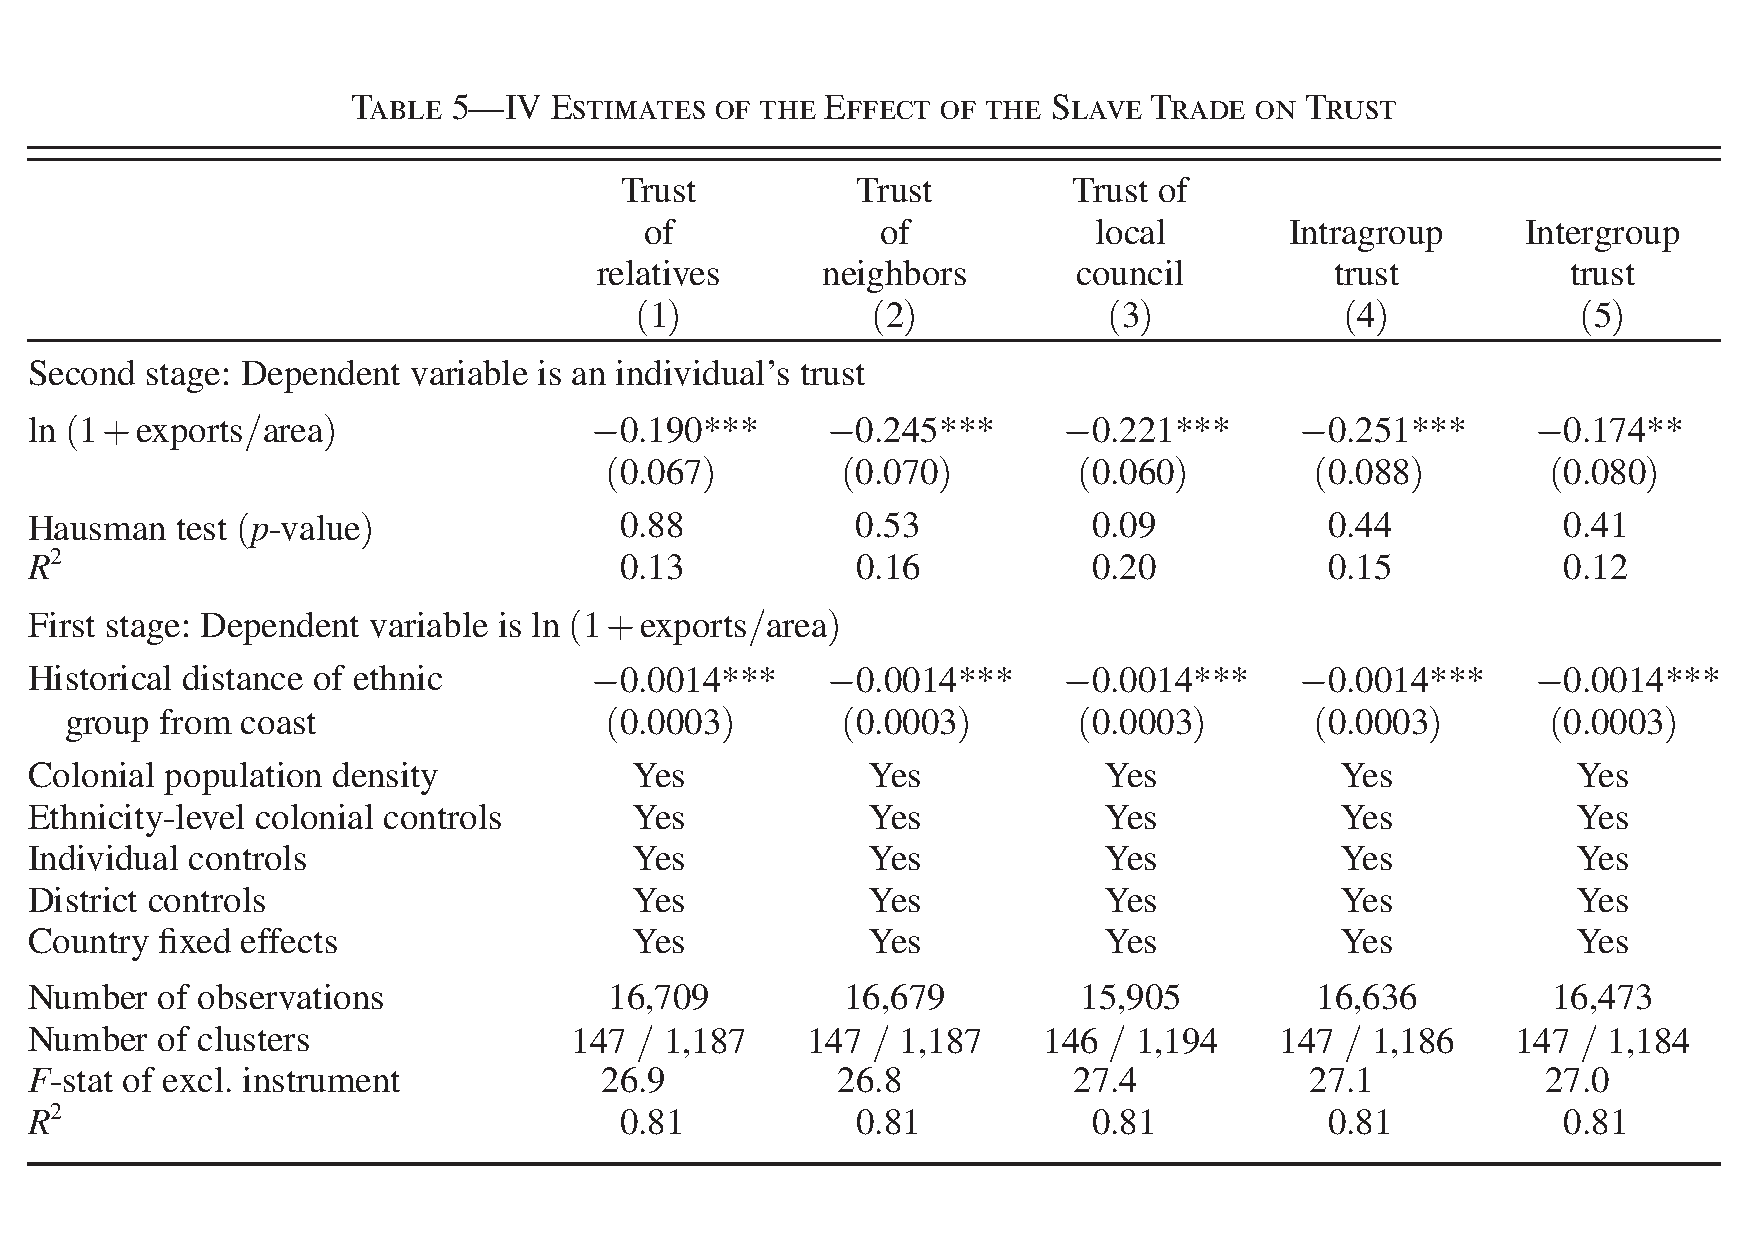
\includegraphics[width=.8\textwidth]{tab5}
	\end{figure}
\end{frame}
%-----------------------------------------------
\begin{frame}{Test de falsificación}
	\begin{itemize}
		\item Usando la encuesta de Asiabarometer, construya una variable dependiente similar a una en una muestra africana;
		\item No se incluyeron covaridades de medidas de ingresos, ocupación y fraccionamiento étnico;
		\item Hipotéticamente, la distancia de la costa para Asia debe ser estadísticamente insignificante. 
	\end{itemize}
\end{frame}
%-----------------------------------------------
\begin{frame}{Test de falsificación}
	\begin{figure}[htb]
		\centering
		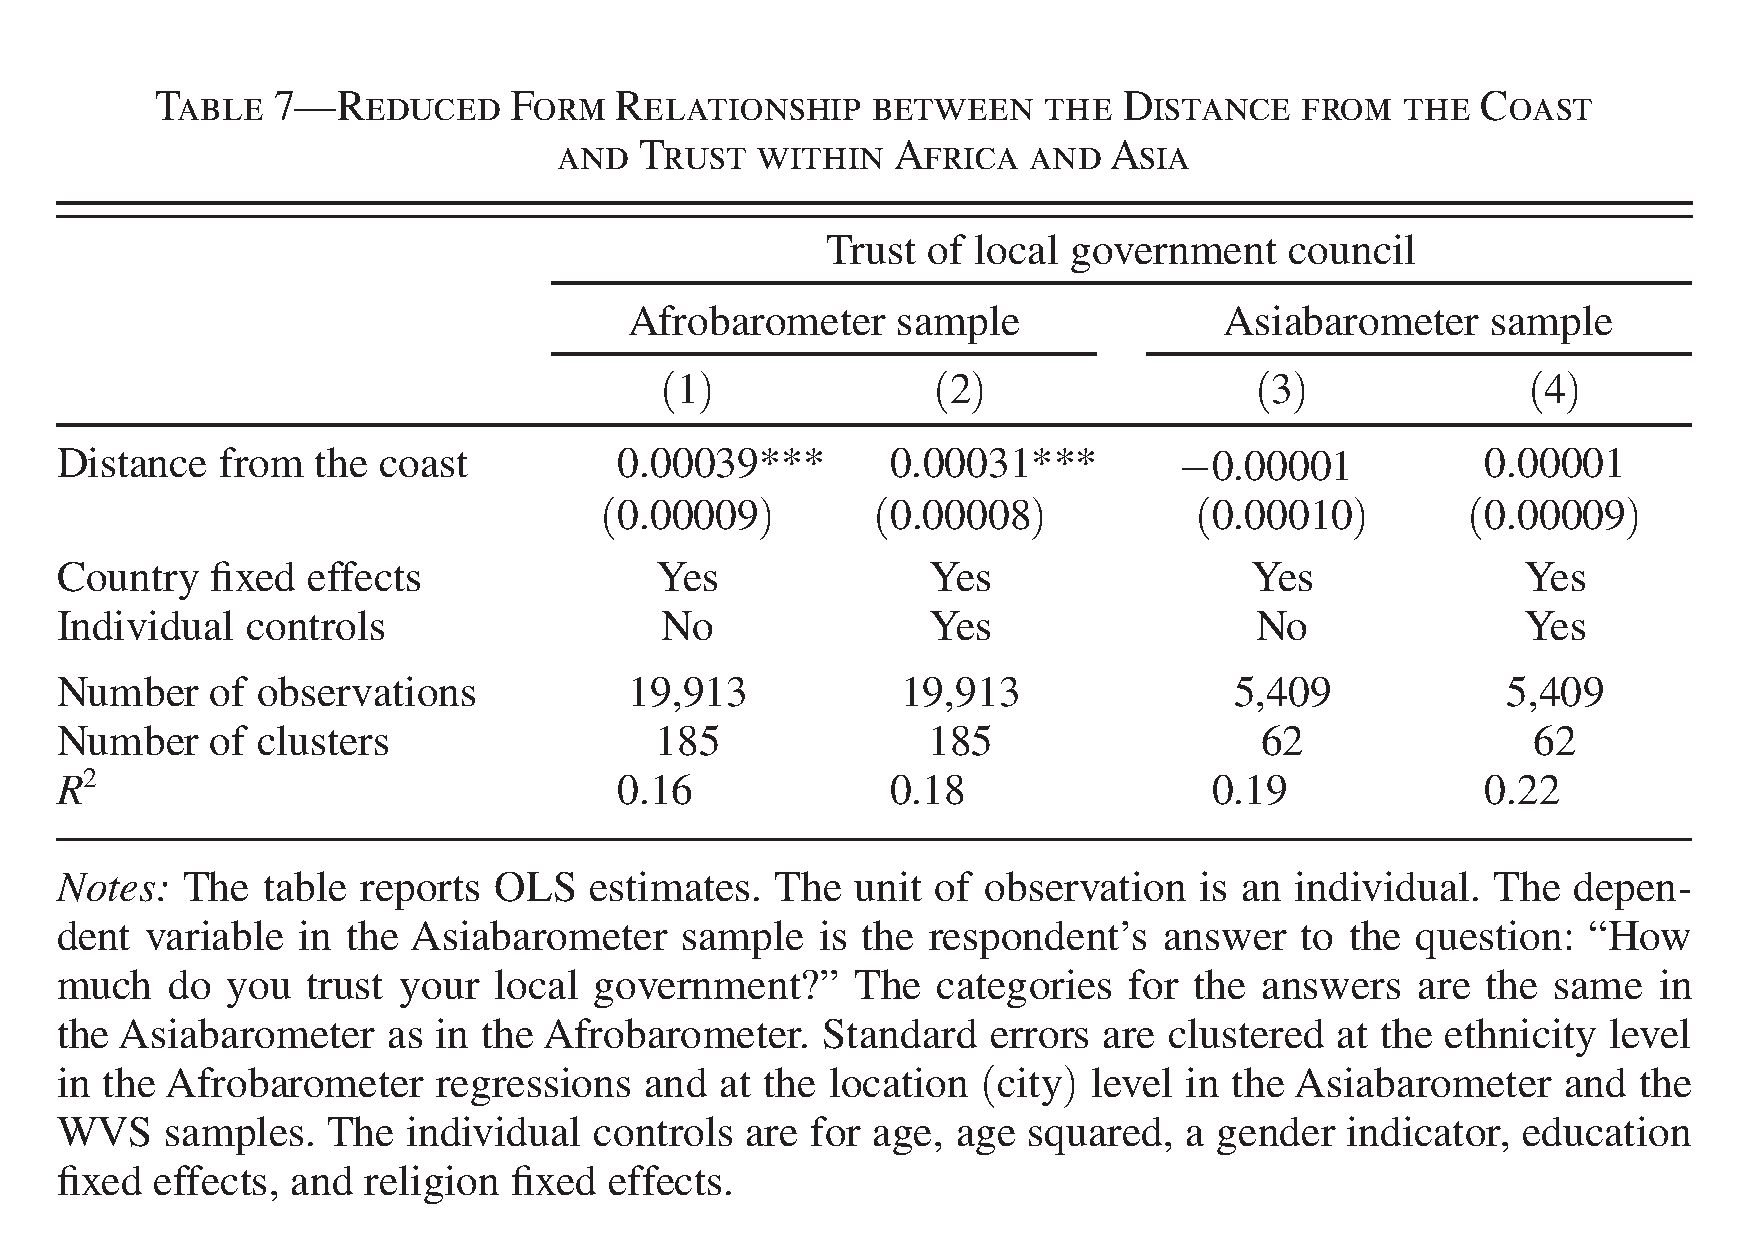
\includegraphics[width=.7\textwidth]{tab7}
	\end{figure}
\end{frame}
%-----------------------------------------------
\begin{frame}{Canales de causalidad}
\begin{itemize}
	\item \textbf{Normas internas: }
	\begin{itemize}
		\item 	la evolución de las normas de comportamiento se vio influenciada durante los 400 años del comercio de esclavos. Aquellos expuestos al comercio se volvieron menos confiados, y sus descendientes siguen siendo menos confiados hoy;
	\end{itemize}
	\item \textbf{Normas externas: }
	\begin{itemize}
		\item el comercio de esclavos se puede correlacionar con una menor confianza en la actualidad porque dio lugar a un deterioro de los estados, instituciones y estructuras legales preexistentes. 
	\end{itemize}
\end{itemize}
\end{frame}
%-----------------------------------------------
\begin{frame}{Pruebas de canales de normas externas e internas}
	\begin{itemize}
		\item Confiabilidad del consejo - medida de la calidad del consejo local;
		\item Bien público: poder de gobierno local de calidad;
		\item La intensidad promedio de las exportaciones de esclavos de las personas pertenecientes a diferentes grupos étnicos que viven en la ciudad, distrito o región del encuestado. 
		\begin{itemize}
			\item La medida está destinada a capturar cualquier efecto del comercio de esclavos en la confiabilidad de otros grupos étnicos que viven cerca del individuo;
		\end{itemize}
		\item Estimar la ecuación principal, controlando las tres medidas de la calidad percibida del consejo local; Calidad del gobierno local.
	\end{itemize}
\end{frame}
%-----------------------------------------------
\begin{frame}{Pruebas de canales de normas externas e internas}
	\begin{figure}[htb]
		\centering
		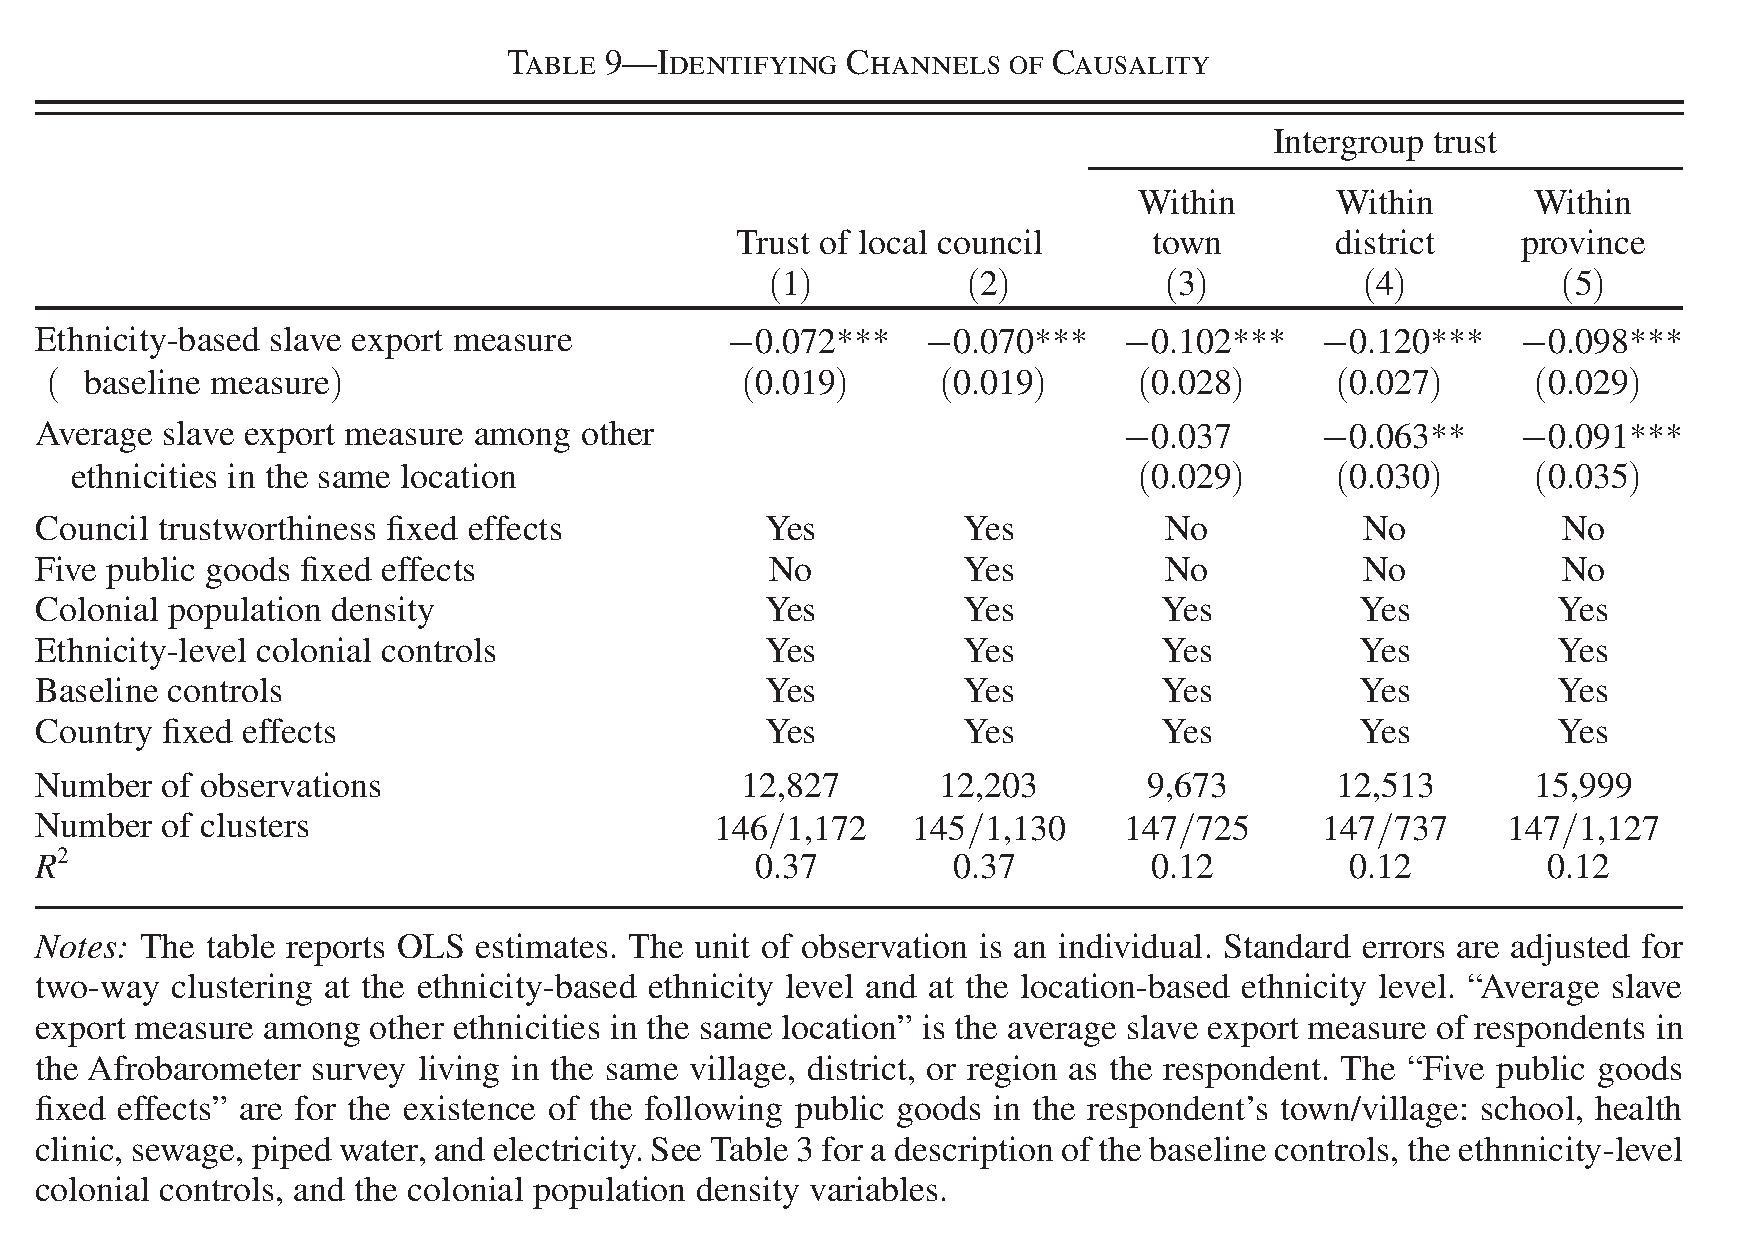
\includegraphics[width=.7\textwidth]{tab9}
	\end{figure}
\end{frame}
%-----------------------------------------------
\begin{frame}{Conclusiones}
	\begin{itemize}
		\item Los bajos niveles de confianza de África se remontan al legado del comercio de esclavos. La confianza de las personas en sus familiares, vecinos, coetnicas y gobiernos locales es menor si sus antepasados se vieron muy afectados por el comercio de esclavos.
		\item Durante los 400 años de inseguridad generados por el comercio de esclavos, las creencias generales o las "reglas de oro" basadas en la desconfianza evolucionaron.
	\end{itemize}
\end{frame}
%-----------------------------------------------
\begin{frame}{Conclusiones}
	\begin{itemize}
		\item El comercio de esclavos dio lugar a un deterioro de las instituciones legales y políticas.
		\item Debido a que estas instituciones debilitadas continúan persistiendo hoy en día, los individuos no están obligados a actuar de manera confiable, y esta falta de confianza resulta en una menor confianza.
	\end{itemize}
\end{frame}
%-----------------------------------------------
\section{Anuncios para la próxima semana}
%-----------------------------------------------
\subsection*{Anuncios para la próxima semana}
%-----------------------------------------------
\begin{frame}{Ensayo grupal}
\begin{itemize}
	\item \textbf{Fecha de Entrega}: 
	\begin{itemize}
		\item Junio 17: 18:00 por el EVA. Entregar solo un archivo pdf. 
	\end{itemize}
	\item \textbf{Idea a discutir}: 
	\begin{itemize}
		\item El tema del ensayo es de elección libre; sin embargo, debe enmarcarse en la segunda unidad.
	\end{itemize}
	\item \textbf{Referencias, esquema y diseño}: 
	\begin{itemize}
		\item Seguir las recomendaciones escritar en la agenda de trabajo. Estilo APA, al menos 2 textos proporcionados por
		mi y 2 investigados por el estudiante. 
	\end{itemize}
	\item \textbf{Extensión y estética}: 
	\begin{itemize}
		\item 3 páginas. Interlineado: sencillo. Fuente: Times New Roman. Tamaño: 12. Margenes: Normales. Ver plantilla. 
	\end{itemize}
\end{itemize}
\end{frame}
%==============================================================
% END
%==============================================================
\miniframesoff 	
\begin{frame}[plain, standout]
Eso es todo por hoy. \\ 
Nos vemos la siguiente semana. 
\end{frame}

\end{document}		
